\documentclass[a4paper]{article}
\usepackage[spanish,es-lcroman]{babel}
\usepackage[utf8]{inputenc}
\spanishdecimal{.}
\usepackage{bm}
\usepackage{amssymb}
\usepackage{mathtools}
\usepackage{amsmath}
\usepackage{geometry}
\usepackage{parskip}
\usepackage{graphicx}
\usepackage{listings}
\usepackage{xcolor}
\usepackage{float}
\usepackage{tikz}
\usepackage{multicol}
\usepackage{enumitem}
\usepackage{subcaption}
\usepackage{animate}
\definecolor{mygreen}{rgb}{0,0.6,0}
\definecolor{mypurple}{rgb}{0.7,0.3,0.7}
\lstset{
	language=Python,
	backgroundcolor=\color{white},
	frame=none,
	%
	basicstyle=\tt,
	commentstyle=\itshape\color{mygreen},
	keywordstyle=\color{magenta},
	identifierstyle=\color{cyan},
	stringstyle=\color{mypurple},
	showstringspaces=false,
	%
	numbers=none,
	%	numberstyle=\color{gray},
	firstnumber = 1,
	stepnumber=2,
	tabsize =2,
	%
	columns=flexible,
	breaklines=true
}
\lstset{
     literate=%
         {á}{{\'a}}1
         {í}{{\'i}}1
         {é}{{\'e}}1
         {ý}{{\'y}}1
         {ú}{{\'u}}1
         {ó}{{\'o}}1
         {ě}{{\v{e}}}1
         {š}{{\v{s}}}1
         {č}{{\v{c}}}1
         {ř}{{\v{r}}}1
         {ž}{{\v{z}}}1
         {ď}{{\v{d}}}1
         {ť}{{\v{t}}}1
         {ň}{{\v{n}}}1
         {ů}{{\r{u}}}1
         {Á}{{\'A}}1
         {Í}{{\'I}}1
         {É}{{\'E}}1
         {Ý}{{\'Y}}1
         {Ú}{{\'U}}1
         {Ó}{{\'O}}1
         {Ě}{{\v{E}}}1
         {Š}{{\v{S}}}1
         {Č}{{\v{C}}}1
         {Ř}{{\v{R}}}1
         {Ž}{{\v{Z}}}1
         {Ď}{{\v{D}}}1
         {Ť}{{\v{T}}}1
         {Ň}{{\v{N}}}1
         {Ů}{{\r{U}}}1      
         {s̄}{{\={s}}}1
         {ñ̄}{{\~{n}}}1
         {Ñ}{{\~{Ñ}}}1
}

\newenvironment{sidefig}[1]
{\noindent\begin{minipage}[c]{#1\textwidth}}
	{\vfill\end{minipage}}
\newcommand{\herefig}[1]{%
\end{minipage}
\hfill
\noindent\begin{minipage}[c]{#1\textwidth} 
	\centering\vfill
}

\author{Celia Rubio Madrigal}
\title{Práctica 7 - GCOMP}
%\date{3 de mayo de 2022}

\begin{document}
	\maketitle
	
	\tableofcontents
	
	\vfill
	
	\begin{center}
		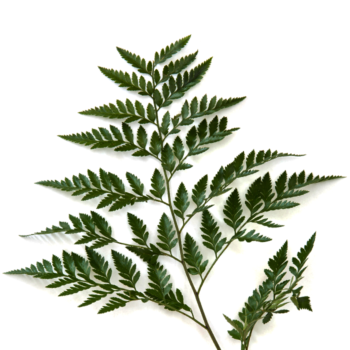
\includegraphics[width=0.45\linewidth]{arbol}
	\end{center}
	
	
	\vfill
	\newpage
	
	\section{Introducción}
	En esta práctica vamos a aplicar la misma transformación isométrica afín a dos sistemas distintos. Esta transformación va a ser la composición de una rotación y una translación.
	
	Este tipo de transformaciones cumplen que mantienen invariantes la distancia entre todos los pares de puntos del sistema. Lo representaremos gráficamente para atestiguarlo.
	
	
	\section{Material usado y metodología}
	En esta práctica, consideraremos solamente la métrica euclídea. 
	
	La rotación será sobre el plano $xy$, y con un ángulo $\theta=3\pi$, sobre el centroide de cada sistema. 
	
	Como buscamos una familia paramétrica en función de un parámetro temporal $t\in[0,1]$, cada fotograma representará una rotación de ángulo $\theta\cdot t$. Es decir, aplicaremos la matriz $M(t)$ al vector $X-C(X)$, donde $C(X)$ es el centroide de $X$, que calculamos mediante \textit{numpy.mean}, y:
	\[ M(t) = \left(\begin{array}{ccc}
	\cos(3\pi\cdot t) & -\sin(3\pi\cdot t) & 0 \\
	\sin(3\pi\cdot t) & \cos(3\pi\cdot t) & 0\\
	0&0&1
	\end{array}\right)\]
	
	Como el centroide queda invariante frente a la rotación, solo queda volver a sumárselo a las cordenadas que se obtienen de la transformación.
	
	Además, aplicaremos una familia paramétrica de translaciones en función de $t$, cuyo vector es: $v(t) = (D(X),D(X),0)$, con $D(X)$ el diámetro mayor del sistema. Lo calculamos aplicando el algoritmo de \textit{ConvexHull} y comparando las distancias entre los vértices de la frontera, en vez de comparar todos los puntos entre sí directamente.
	
	\subsection{Apartado \textit{i})}
	En el primer apartado, aplicaremos la transformación afín $T(t) = M(t) \cdot X + v(t)$ a los puntos generados por la función $axes3d.get\_test\_data(0.05)$.
	
	\subsection{Apartado \textit{ii})}
	En el segundo apartado, aplicaremos la transformación afín $T(t)$ a una imagen digital. En concreto, tomaremos la imagen \textit{arbol.png}, que tiene como variables de estado el plano \textit{xy} y los colores \textit{rgb}. Consideraremos el subsistema dado por los valores de la imagen cuya coordenada roja \textit{r} sea menor que 240.
	
	\section{Resultados y conclusiones}
	
	\subsection{Apartado \textit{i})}
	Para el primer sistema, su diámetro mayor es de $159.65 \pm 0.01$, y su centroide se encuentra en las coordenadas $[-0.25,-0.25,-1.28] \pm 0.01$.
	
	A continuación\footnote{Para ver ambos gráficos en movimiento, se recomienda abrir este PDF en Adobe Reader u Okular.}, y así como en los archivos adjuntos, se encuentra la animación de la sucesión de transformaciones paramétricas $T(t)$ sobre este sistema.
	
	\begin{center}
		\animategraphics[method=ocg,width=0.33\paperwidth,loop,autoplay]{6}{img/1_}{1}{40}
	\end{center}
	
	
	\subsection{Apartado \textit{ii})}
	Para el segundo sistema, dejaremos invariantes las coordenadas de color y solo transformaremos \textit{xy}. El diámetro es de $357.41 \pm 0.01$ y su centroide se encuentra en $[173.48, 204.16] \pm 0.01$. Dibujaremos, además, la figura en el espacio tridimensional, poniendo su coordenada de altura a 0.
	
	A continuación\footnote{Para ver ambos gráficos en movimiento, se recomienda abrir este PDF en Adobe Reader u Okular.}, y así como en los archivos adjuntos, se encuentra la animación de la sucesión de transformaciones paramétricas $T(t)$ sobre este sistema. Hemos coloreado de azul el punto origen, y de rojo el centroide original.
	
	\begin{center}
		\animategraphics[method=ocg,width=0.33\paperwidth,loop,autoplay]{6}{img/2_}{1}{40}
	\end{center}
	
	Mediante estos ejemplos, hemos calculado y averiguado cómo se transforman sistemas de tal manera que no se deformen las distancias entre sus puntos. Así, las animaciones obtenidas simulan objetos rígido moviéndose por el espacio.
	
	
	\newpage
	\section{Código}\label{codigo}
	
	\lstinputlisting[language=Python]{p7_rubiomadrigalcelia.py}
	
\end{document}
